\documentclass{article}
\usepackage{amsmath}
\usepackage{amssymb}
\usepackage{graphicx}
\usepackage{hyperref}
\usepackage[version=4]{mhchem}


\begin{document}
(1975 AMC) In the adjoining figure triangle \(A B C\) is such that \(A B=4\) and \(A C=8\). If \(M\) is the midpoint of \(B C\) and \(A M=3\), what is the length of \(B C\) ?\\
(A) \(2 \sqrt{26}\)\\
(B) \(2 \sqrt{31}\)\\
(C) 9\\
(D) \(4+2 \sqrt{13}\)\\
(E) not enough information given to solve the problem\\
\centering
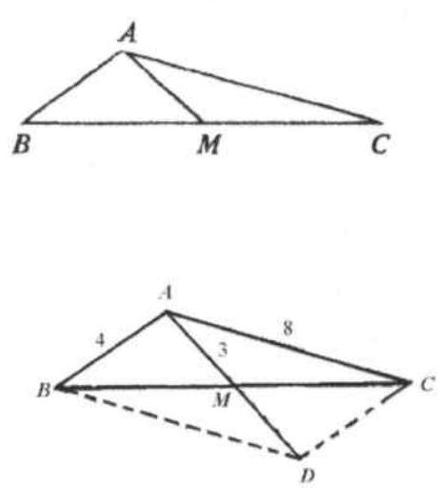
\includegraphics[width=\textwidth]{images/026(2).jpg}

Solution: (B).\\
Extend \(A M\) to \(D\) such that \(A M=M D\). Connect \(B D\) and \(C D . A B D C\) is a parallelogram.

We know that the sum of the squares of the sides of a parallelogram is equal to the sum of the squares of its diagonals.

Applying this to the parallelogram having \(A B\) and \(A C\) as adjacent sides yields\\
\(A D^{2}+B C^{2}=A B^{2}+C D^{2}+A C^{2}+B D^{2} \Rightarrow A D^{2}+B C^{2}=2\left(A B^{2}+A C^{2}\right)\)\\
\(B C^{2}=2\left(4^{2}+8^{2}\right)-6^{2}=124 . \quad B C=2 \sqrt{31}\).
\end{document}
